
<<<<<<< HEAD
\chapter{Fractional step method (FSM)}

In this Chapter

Hereinafter, it is assumed that the studied problems occur in a contractible bounded open set $\Omega \subset \real^3$ with smooth boundary. Besides, these problems last for finite time, that is to say, the time interval is $I = [t_0, t_f] \subset \real$.




\section{First approach to the FSM}

\subsection{Time integration of the Navier--Stokes equations}

<<<<<<< HEAD
Recall that the Navier--Stokes equations for incompressible and constant viscosity flows are
=======
Recall that the Navier--Stokes equations for incompressible and constant viscosity flows are given by
>>>>>>> Changes in report. Changes in code: redefinition of surfX, surfY, vol
\begin{equation} \label{eq:navier_stokes_01}
    \left\{
    \begin{aligned}
        \div{\vb{v}} &= 0 \\
        \rho \pdv{\vb{v}}{t} + (\rho \vb{v} \vdot \grad) \vb{v} &= -\grad{p} + \mu \laplacian{\vb{v}}
    \end{aligned}
    \right.
\end{equation}
<<<<<<< HEAD
where $\vb{u} = u \vb{i} + v \vb{j} + w \vb{k}$. By defining the operator
\begin{equation}
    \vb{R}(\vb{v}) = \mu \laplacian{\vb{v}} - (\rho \vb{v} \vdot \grad) \vb{v}
\end{equation}
\eqref{eq:navier_stokes_01} may be rewritten as follows:
=======
where $\rho$ and $\mu$ are the fluid density and viscosity, respectively, $p \colon \Omega \times I \rightarrow \real$ is the pressure field and $\vb{v} = (u, v, w) \colon \Omega \times I \rightarrow \real^3$ is the velocity field. The operator
\begin{equation}
    \vb{R}(t,\vb{v}) = 
    \mu \laplacian{\vb{v}(\cdot,t)} - (\rho \vb{v}(\cdot,t) \vdot \grad) \vb{v}(\cdot,t) =
    \mu \laplacian{\vb{v}} - (\rho \vb{v} \vdot \grad) \vb{v}
\end{equation}
permits rewriting Equation \eqref{eq:navier_stokes_01} as follows:
>>>>>>> Changes in report. Changes in code: redefinition of surfX, surfY, vol
\begin{equation} \label{eq:navier_stokes_02}
    \left\{
    \begin{aligned}
        \div{\vb{v}} &= 0 \\
<<<<<<< HEAD
        \rho \pdv{\vb{v}}{t} &= \vb{R}(\vb{v}) - \grad{p}
    \end{aligned}
    \right.
\end{equation}

\colorbox{red}{why integrate the equations?}

Let $[t^n, t^{n+1}] \subset [t_0, t_f]$ be a non--degenerate time interval with $\Delta t = t^{n+1} - t^n$. An implicit integration scheme ($\beta = 1$) is used to integrate the continuity equation with respect to time:
\begin{gather*}
    \int_{t^n}^{t^{n+1}} \div{\vb{v}} \dd{t} =
    \left( \beta \div{\vb{v}}^{n+1} + (1 - \beta) \div{\vb{v}}^{n} \right) \, \Delta t =
    \div{\vb{v}}^{n+1} \, \Delta t = 0
\end{gather*}
Since $\Delta t > 0$, it follows that
\begin{equation} \label{eq:continuity_time_integrated}
    \div{\vb{v}}^{n+1} = 0
=======
        \rho \pdv{\vb{v}}{t} &= \vb{R}(t,\vb{v}) - \grad{p}
    \end{aligned}
    \right.
\end{equation}
Therefore the momentum equation is now an evolution equation.

In order to solve \eqref{eq:navier_stokes_02} numerically in $\Omega \times I \subset \real^4$ with suitable boundary conditions on $\partial \Omega$ and initial conditions on $\Omega \times \{ t = 0 \}$ following a finite volume method, it is necessary to discretise $\Omega$ in control volumes and integrate \eqref{eq:navier_stokes_02} over time intervals of the form $[t^n, t^{n+1}]$. 


Let $[t^n, t^{n+1}] \subset [t_0, t_f] = \overline{I}$ be a non--degenerate time interval and $\Delta t = t^{n+1} - t^n$. An implicit integration scheme ($\beta = 1$) is used to integrate the continuity equation with respect to time:
\begin{gather*}
    \int_{t^n}^{t^{n+1}} \div{\vb{v}} \dd{t} =
    \left( \beta (\div{\vb{v}})^{n+1} + (1 - \beta) (\div{\vb{v}})^{n} \right) \, \Delta t =
    (\div{\vb{v}})^{n+1} \, \Delta t = 0
\end{gather*}
Since $\Delta t > 0$, it follows that
\begin{equation} \label{eq:continuity_time_integrated}
    (\div{\vb{v}})^{n+1} \approx \div{\vb{v}^{n+1}} = 0
>>>>>>> Changes in report. Changes in code: redefinition of surfX, surfY, vol
\end{equation}
which is the time--integrated continuity equation. As for the momentum equation,
\begin{equation*}
    \int_{t^n}^{t^{n+1}} \rho \pdv{\vb{v}}{t} \dd{t} =
    \int_{t^n}^{t^{n+1}} \vb{R}(\vb{v}) \dd{t} -
    \int_{t^n}^{t^{n+1}} \grad{p} \dd{t}
\end{equation*}
<<<<<<< HEAD
The left--hand side computation is straightforward as the density is constant and the fundamental theorem of calculus is applied:
=======
For the left--hand side, it is known that the density is constant, hence:
>>>>>>> Changes in report. Changes in code: redefinition of surfX, surfY, vol
\begin{equation*}
    \int_{t^n}^{t^{n+1}} \rho \pdv{\vb{v}}{t} \dd{t} =
    \rho \int_{t^n}^{t^{n+1}} \pdv{\vb{v}}{t} \dd{t} =
    \rho ( \vb{v}^{n+1} - \vb{v}^n )
\end{equation*}
In order to integrate $\vb{R}(\vb{v})$, define
\begin{equation*}
<<<<<<< HEAD
    \mathfrak{R}(\vb{v},t) = \int_{t_0}^s \vb{R}(\vb{v}) \dd{s}
\end{equation*}
so that
\begin{equation} \label{eq:integral_Rv}
    \mathfrak{R}(\vb{v},t^{n+1}) - \mathfrak{R}(\vb{v},t^{n}) =
    \int_{t^n}^{t^{n+1}} \vb{R}(\vb{v}) \dd{t}
\end{equation}
By applying the two--step Adams--Bashforth method, \eqref{eq:integral_Rv} results in
\begin{equation*}
    \int_{t^n}^{t^{n+1}} \vb{R}(\vb{v}) \dd{t} =
    \left( \frac{3}{2} \vb{R}(\vb{v}^{n+1}) - \frac{1}{2} \vb{R}(\vb{v}^n) \right) \, \Delta t
\end{equation*}
Again the implicit integration scheme ($\beta = 1$) is used to compute the third term:
=======
    \mathfrak{R}(t,\vb{v}) = \int_{0}^t \vb{R}(s,\vb{v}) \dd{s}
\end{equation*}
so that
\begin{equation} \label{eq:integral_Rv}
    \mathfrak{R}(t^{n+1}, \vb{v}) - \mathfrak{R}(t^n, \vb{v}) =
    \int_{t^n}^{t^{n+1}} \vb{R}(s,\vb{v}) \dd{s}
\end{equation}
By applying the two--step Adams--Bashforth method, \eqref{eq:integral_Rv} results in
\begin{equation*}
    \int_{t^n}^{t^{n+1}} \vb{R}(s,\vb{v}) \dd{t} =
    \left( \frac{3}{2} \vb{R}(t^{n}, \vb{v}) - \frac{1}{2} \vb{R}(t^{n-1}, \vb{v}) \right) \, \Delta t
\end{equation*}
For the sake of simplicity in notation, it shall be written $\vb{R}(\vb{v}^n)$ in place of $\vb{R}(t^n, \vb{v})$. Regarding the integral of the pressure gradient, again the implicit integration scheme ($\beta = 1$) is used, which yields
>>>>>>> Changes in report. Changes in code: redefinition of surfX, surfY, vol
\begin{equation*}
    \int_{t^n}^{t^{n+}} \grad{p} \dd{t} =
    \left( \beta \grad{p}^{n+1} + (1 - \beta) \grad{p}^n \right) \, \Delta t =
    \grad{p}^{n+1} \, \Delta t
\end{equation*}
<<<<<<< HEAD
Rearranging terms yields the time--integrated momentum equation:
\begin{equation}
    \rho \frac{\vb{v}^{n+1} - \vb{v}^n}{\Delta t} =
    \frac{3}{2} \vb{R}(\vb{v}^{n+1}) - \frac{1}{2} \vb{R}(\vb{v}^n) - \grad{p}^{n+1}
\end{equation}
=======
By rearranging terms the time--integrated momentum equation is obtained:
\begin{equation} \label{eq:momentum_time_integrated}
    \rho \frac{\vb{v}^{n+1} - \vb{v}^n}{\Delta t} =
    \frac{3}{2} \vb{R}(\vb{v}^{n}) - \frac{1}{2} \vb{R}(\vb{v}^{n-1}) - \grad{p}^{n+1}
\end{equation}

\subsection{Application of the Helmholtz decomposition to the Navier--Stokes equations}

Define the predictor velocity by
\begin{equation} \label{eq:predictor_velocity}
    \vb{v}^p = \vb{v}^{n+1} + \frac{\Delta t}{\rho} \grad{p^{n+1}}
\end{equation}

\colorbox{red}{Since the velocity field is divergence--less, the predictor velocity is decomposed into... which is unique}

After introducing \eqref{eq:predictor_velocity} into \eqref{eq:momentum_time_integrated}, the time--integrated momentum equation becomes the velocity projection equation:
\begin{equation} \label{eq:momentum_time_integrated_predictor_velocity}
    \rho \frac{\vb{v}^p - \vb{v}^n}{\Delta t} = 
    \frac{3}{2} \vb{R}(\vb{v}^n) - \frac{1}{2} \vb{R}(\vb{v}^{n-1})
\end{equation}

Taking the divergence of both sides of \eqref{eq:predictor_velocity} and using \eqref{eq:continuity_time_integrated} results in
\begin{equation}
    \div{\vb{v}^p} = 
    \div{\vb{v}^{n+1}} + \div(\frac{\Delta t}{\rho} \grad{p}^{n+1}) = 
    \frac{\Delta t}{\rho} \laplacian{p^{n+1}}
\end{equation}
which is a Poisson equation for the pressure term:
\begin{equation} \label{eq:poisson_equation_pressure}
    \laplacian{p^{n+1}} = \frac{\rho}{\Delta t} \div{\vb{v}^p}
\end{equation}

\subsection{Solving algorithm}

Notice that from Equation \eqref{eq:momentum_time_integrated_predictor_velocity} the predictor velocity may also be calculated by
\begin{equation} \label{eq:predictor_velocity_2}
    \vb{v}^p = 
    \vb{v}^n + 
    \frac{\Delta t}{\rho} \left( \frac{3}{2} \vb{R}(\vb{v}^n) - \frac{1}{2} \vb{R}(\vb{v}^{n-1}) \right)
\end{equation}
Assume that the data up to time $t^n$ is known, that is to say, $\vb{R}(\vb{v}^{n-1}), \vb{R}(\vb{v}^n)$ and $\vb{v}^n$ are known. Then the computation of the predictor velocity is immediate by means of Equation \eqref{eq:predictor_velocity_2}. By integrating the laplacian of the pressure term at $t^{n+1}$ on each control volume, equation \eqref{eq:poisson_equation_pressure} may be transformed into a linear equation which, with suitable boundary conditions on $\partial \Omega$, allows us to compute $p^{n+1}$ (this matter is carried out in Section \colorbox{red}{section}). As a result, both $\vb{v}^p$ and $\grad{p}^{n+1}$ are known, whereby the velocity field at $t^{n+1}$ is obtained from Equation \eqref{eq:predictor_velocity}:
\begin{equation} \label{eq:velocity_at_next_instant}
    \vb{v}^{n+1} = \vb{v}^p - \frac{\Delta t}{\rho} \grad{p^{n+1}}
\end{equation} 
This procedure is summarised in the following algorithm:
\begin{algorithm}[ht]
	\caption{Computation of the velocity field at $t^{n+1}$.}
	\label{algorithm:computation_of_velocity_field_at_next_instant}
	\begin{algorithmic}[0]
		\State 
		\begin{enumerate}[label=\textbf{\arabic*},topsep=0pt]
			\item Evaluation of $\vb{R}(\vb{v}^n)$.
			\item Evaluation of the predictor velocity $\vb{v}^p$ with Equation \eqref{eq:predictor_velocity_2}.
			\item Evaluation of the pressure at $t^{n+1}$ by solving Equation \eqref{eq:poisson_equation_pressure}.
			\item Evaluation of the velocity at $t^{n+1}$ with Equation \eqref{eq:velocity_at_next_instant}.
		\end{enumerate}
	\end{algorithmic}
\end{algorithm}

Despite of the simplicity Algorithm \ref{algorithm:computation_of_velocity_field_at_next_instant}, the produced velocity and pressure fields entail a fundamental problem, namely, these have no physical meaning. In the section below, an example of this is exposed.




>>>>>>> Changes in report. Changes in code: redefinition of surfX, surfY, vol

% <<<<<<< HEAD
\subsection{The checkerboard problem}

Notice that \eqref{eq:velocity_time_n+1_fsm_first_approach} is a vector equation, hence expanding it by components gives:
\begin{equation} \label{eq:velocity_checkerboard_problem}
    \left\{
        \begin{aligned}
            u^{n+1} &= u^p - \frac{\Delta t}{\rho} p_x^{n+1} \\
            v^{n+1} &= v^p - \frac{\Delta t}{\rho} p_y^{n+1} \\
            w^{n+1} &= w^p - \frac{\Delta t}{\rho} p_z^{n+1} \\
        \end{aligned}
    \right.
\end{equation}
Consider the discretization of the $x$--component of \eqref{eq:velocity_checkerboard_problem}:
\begin{equation}
    u_P^{n+1} = 
    u_P^p - \frac{\Delta t}{\rho} 
    \left( \frac{p_E^{n+1} - p_W^{n+1}}{2 \, \Delta x} \right)
\end{equation}
Notice that the discrete approximation of $\grad{p}^{n+1}$ is independent of $p_P^{n+1}$.

=======
\section{The checkerboard problem}

Consider the $x$--component of Equation \eqref{eq:velocity_at_next_instant}
\begin{equation} \label{eq:velocity_at_next_instant_x_component}
    u^{n+1} = 
    u^p - \frac{\Delta t}{\rho} \left( \pdv{p}{x} \right)^{n+1} \approx
    u^p - \frac{\Delta t}{\rho} \pdv{p^{n+1}}{x}
\end{equation}
and the following discretisation in the $x$--direction of a neighbourhood of a point $P$:
>>>>>>> Changes in report. Changes in code: redefinition of surfX, surfY, vol
\begin{figure}[h]
    \centering
    \begin{tikzpicture}
        \def\side{2cm}
        \def\ys{0.5cm}
        \def\ofset{0.1cm}
<<<<<<< HEAD
        \def\arrowlength{0.75cm}
=======
        \def\velocitylength{0.75cm}
>>>>>>> Changes in report. Changes in code: redefinition of surfX, surfY, vol
        % Control volume
        \fill[cvfill] (0,0) rectangle (3*\side,\side);
        \draw[wall] (0,0) rectangle (3*\side,\side);
        \draw[wall] (\side,0) -- ++(0,\side);
        \draw[wall] (2*\side,0) -- ++(0,\side);
        % Node W
<<<<<<< HEAD
        \draw[velocity] (0.5*\side,0.5*\side) -- node[midway, below]{$u_W^{n+1}$} ++(\arrowlength,0);
        \filldraw[black] (0.5*\side,0.5*\side) circle (2pt);
        \node[black, yshift=+\ys] at (0.5*\side,0.5*\side) {$p_W^{n+1}$};
        % Node P
        \draw[velocity] (1.5*\side,0.5*\side) -- node[midway, below]{$u_P^{n+1}$} ++(\arrowlength,0);
        \filldraw[black] (1.5*\side,0.5*\side) circle (2pt);
        \node[black, yshift=+\ys] at (1.5*\side,0.5*\side) {$p_P^{n+1}$};
        % Node E
        \draw[velocity] (2.5*\side,0.5*\side) -- node[midway, below]{$u_E^{n+1}$} ++(\arrowlength,0);
=======
        \draw[velocity] (0.5*\side,0.5*\side) -- node[midway, below]{$u_W^{n+1}$} ++(\velocitylength,0);
        \filldraw[black] (0.5*\side,0.5*\side) circle (2pt);
        \node[black, yshift=+\ys] at (0.5*\side,0.5*\side) {$p_W^{n+1}$};
        % Node P
        \draw[velocity] (1.5*\side,0.5*\side) -- node[midway, below]{$u_P^{n+1}$} ++(\velocitylength,0);
        \filldraw[black] (1.5*\side,0.5*\side) circle (2pt);
        \node[black, yshift=+\ys] at (1.5*\side,0.5*\side) {$p_P^{n+1}$};
        % Node E
        \draw[velocity] (2.5*\side,0.5*\side) -- node[midway, below]{$u_E^{n+1}$} ++(\velocitylength,0);
>>>>>>> Changes in report. Changes in code: redefinition of surfX, surfY, vol
        \filldraw[black] (2.5*\side,0.5*\side) circle (2pt);
        \node[black, yshift=+\ys] at (2.5*\side,0.5*\side) {$p_E^{n+1}$};
        % Measuring line
        \draw[measureline] (0.5*\side,-0.5*\side) -- node[above]{$\Delta x$} ++(\side,0);
        \draw[measureline] (1.5*\side,-0.5*\side) -- node[above]{$\Delta x$} ++(\side,0);
        \draw[measureaux, yshift=-\ofset] (0.5*\side,-0.5*\side) -- ++(0,0.5*\side);
        \draw[measureaux, yshift=-\ofset] (1.5*\side,-0.5*\side) -- ++(0,0.5*\side);
        \draw[measureaux, yshift=-\ofset] (2.5*\side,-0.5*\side) -- ++(0,0.5*\side);
    \end{tikzpicture}
<<<<<<< HEAD
\end{figure}

=======
    \caption{}
    \label{fig:checkerboard_problem_figure_1}
\end{figure}

By applying finite differences at $P$ to compute the partial derivative in Equation \eqref{eq:velocity_at_next_instant_x_component}, one may approximate $u_P^{n+1}$ as follows:
\begin{equation}
    u_P^{n+1} = u^p - \frac{\Delta t}{\rho} \frac{p_E^{n+1} - p_W^{n+1}}{2 \Delta x}
\end{equation}
We notice that $u_P^{n+1}$ does not depend upon $p_P^{n+1}$. The same is true for the $y$ and $z$--components of \eqref{eq:velocity_at_next_instant}. This is a consequence of the pressure $p_P^{n+1}$ and the gradient $\grad{p}^{n+1}$ being decoupled, \ie independent of one another.

This leads to converged velocity fields for unphysical pressure distributions. For instance, consider the following situation
>>>>>>> Changes in report. Changes in code: redefinition of surfX, surfY, vol

\begin{figure}[h]
    \centering
    \begin{tikzpicture}
        \def\side{2cm}
        \def\ys{0.5cm}
        \def\ofset{0.1cm}
<<<<<<< HEAD
        \def\arrowlength{0.75cm}
=======
        \def\velocitylength{0.75cm}
>>>>>>> Changes in report. Changes in code: redefinition of surfX, surfY, vol
        % Control volumes
        \fill[cvfill] (0,0) rectangle (5*\side,\side);
        \draw[wall] (0,0) rectangle (5*\side,\side);
        \draw[wall] (\side,0) -- ++(0,\side);
        \draw[wall] (2*\side,0) -- ++(0,\side);
        \draw[wall] (3*\side,0) -- ++(0,\side);
        \draw[wall] (4*\side,0) -- ++(0,\side);



        % Node WW
        \begin{scope}[shift={(0.5*\side, 0.5*\side)}]
<<<<<<< HEAD
            \draw[velocity] (0,0) -- node[midway, below]{$u_{WW}^{n+1}$} ++(\arrowlength,0);
            \filldraw[black] (0,0) circle (2pt);
            \node[black, yshift=+\ys] at (0,0) {$p_{WW}^{n+1}$};
        \end{scope}

        
        % Node P
        \draw[velocity] (1.5*\side,0.5*\side) -- node[midway, below]{$u_P^{n+1}$} ++(\arrowlength,0);
        \filldraw[black] (1.5*\side,0.5*\side) circle (2pt);
        \node[black, yshift=+\ys] at (1.5*\side,0.5*\side) {$p_P^{n+1}$};
        % Node E
        \draw[velocity] (2.5*\side,0.5*\side) -- node[midway, below]{$u_E^{n+1}$} ++(\arrowlength,0);
        \filldraw[black] (2.5*\side,0.5*\side) circle (2pt);
        \node[black, yshift=+\ys] at (2.5*\side,0.5*\side) {$p_E^{n+1}$};
    \end{tikzpicture}
\end{figure}
=======
            \draw[velocity] (0,0) -- node[midway, below]{$u_{WW}^{n+1}$} ++(\velocitylength,0);
            \filldraw[black] (0,0) circle (2pt);
            \node[black, yshift=+\ys] at (0,0) {$p_{WW}^{n+1}$};
        \end{scope}
        
        % Node W
        \begin{scope}[shift={(1.5*\side,0.5*\side)}]
            \draw[velocity] (0,0) -- node[midway, below]{$u_{W}^{n+1}$} ++(\velocitylength,0);
            \filldraw[black] (0,0) circle (2pt);
            \node[black, yshift=+\ys] at (0,0) {$p_{W}^{n+1}$};
        \end{scope}
        
        % Node P
        \begin{scope}[shift={(2.5*\side,0.5*\side)}]
            \draw[velocity] (0,0) -- node[midway, below]{$u_{P}^{n+1}$} ++(\velocitylength,0);
            \filldraw[black] (0,0) circle (2pt);
            \node[black, yshift=+\ys] at (0,0) {$p_{P}^{n+1}$};
        \end{scope}
        
        % Node E
        \begin{scope}[shift={(3.5*\side,0.5*\side)}]
            \draw[velocity] (0,0) -- node[midway, below]{$u_{E}^{n+1}$} ++(\velocitylength,0);
            \filldraw[black] (0,0) circle (2pt);
            \node[black, yshift=+\ys] at (0,0) {$p_{E}^{n+1}$};
        \end{scope}
        
        % Node EE
        \begin{scope}[shift={(4.5*\side,0.5*\side)}]
            \draw[velocity] (0,0) -- node[midway, below]{$u_{EE}^{n+1}$} ++(\velocitylength,0);
            \filldraw[black] (0,0) circle (2pt);
            \node[black, yshift=+\ys] at (0,0) {$p_{EE}^{n+1}$};            
        \end{scope}

        \begin{scope}[shift={(5*\side,0.5*\side)}]
            \node[anchor=west] at (0,0) {
                \begin{tabular}{c}
                    $p_{WW}^{n+1} = p_{P}^{n+1} = p_{EE}^{n+1} = 100$ \\
                    $p_{W}^{n+1} = p_{E}^{n+1} = 0$
                \end{tabular}
            };
        \end{scope}
    \end{tikzpicture}
    \caption{}
    \label{fig:checkerboard_problem_figure_2}
\end{figure}

which is a checkerboard pattern as far as the pressure distribution is concerned. The partial derivative of pressure satisfies $\partial_x p^{n+1} = 0$ at nodes $W$, $P$ and $E$, despite being a pressure distribution with no physical sense, thus yielding incorrect converged velocities at these nodes. It is clear that a more sophisticated strategy to relate the velocity and pressure fields is needed. 



>>>>>>> Changes in report. Changes in code: redefinition of surfX, surfY, vol

=======
\chapter{Fractional Step Method}

In this Chapter the Fractional Step Method (FSM) is introduced and justified. \colorbox{red}{asdsadas}

Hereinafter, it is assumed that the studied PDEs occur in a bounded open set $\Omega \subset \real^3$ with boundary as smooth as necessary, and last for finite time, that is to say, the time interval is $I = (0, t_\text{max}) \subset \real$ with $t_\text{max} > 0$.



\section{First approach to the FSM}

\subsection{Time integration of the Navier--Stokes equations}

<<<<<<< HEAD
Recall that the Navier--Stokes equations for incompressible and constant viscosity flows are
=======
Recall that the Navier--Stokes equations for incompressible and constant viscosity flows are given by
>>>>>>> Changes in report. Changes in code: redefinition of surfX, surfY, vol
\begin{equation} \label{eq:navier_stokes_01}
    \left\{
    \begin{aligned}
        \div{\vb{v}} &= 0 \\
        \rho \pdv{\vb{v}}{t} + (\rho \vb{v} \vdot \grad) \vb{v} &= -\grad{p} + \mu \laplacian{\vb{v}}
    \end{aligned}
    \right.
\end{equation}
<<<<<<< HEAD
where $\vb{u} = u \vb{i} + v \vb{j} + w \vb{k}$. By defining the operator
\begin{equation}
    \vb{R}(\vb{v}) = \mu \laplacian{\vb{v}} - (\rho \vb{v} \vdot \grad) \vb{v}
\end{equation}
\eqref{eq:navier_stokes_01} may be rewritten as follows:
=======
where $\rho$ and $\mu$ are the fluid density and viscosity, respectively, $p \colon \Omega \times I \rightarrow \real$ is the pressure field and $\vb{v} = (u, v, w) \colon \Omega \times I \rightarrow \real^3$ is the velocity field. The operator
\begin{equation}
    \vb{R}(t,\vb{v}) = 
    \mu \laplacian{\vb{v}(\cdot,t)} - (\rho \vb{v}(\cdot,t) \vdot \grad) \vb{v}(\cdot,t) =
    \mu \laplacian{\vb{v}} - (\rho \vb{v} \vdot \grad) \vb{v}
\end{equation}
permits rewriting Equation \eqref{eq:navier_stokes_01} as follows:
>>>>>>> Changes in report. Changes in code: redefinition of surfX, surfY, vol
\begin{equation} \label{eq:navier_stokes_02}
    \left\{
    \begin{aligned}
        \div{\vb{v}} &= 0 \\
<<<<<<< HEAD
        \rho \pdv{\vb{v}}{t} &= \vb{R}(\vb{v}) - \grad{p}
    \end{aligned}
    \right.
\end{equation}

\colorbox{red}{why integrate the equations?}

Let $[t^n, t^{n+1}] \subset [t_0, t_f]$ be a non--degenerate time interval with $\Delta t = t^{n+1} - t^n$. An implicit integration scheme ($\beta = 1$) is used to integrate the continuity equation with respect to time:
\begin{gather*}
    \int_{t^n}^{t^{n+1}} \div{\vb{v}} \dd{t} =
    \left( \beta \div{\vb{v}}^{n+1} + (1 - \beta) \div{\vb{v}}^{n} \right) \, \Delta t =
    \div{\vb{v}}^{n+1} \, \Delta t = 0
\end{gather*}
Since $\Delta t > 0$, it follows that
\begin{equation} \label{eq:continuity_time_integrated}
    \div{\vb{v}}^{n+1} = 0
=======
        \rho \pdv{\vb{v}}{t} &= \vb{R}(t,\vb{v}) - \grad{p}
    \end{aligned}
    \right.
\end{equation}
Therefore the momentum equation is now an evolution equation.

In order to solve \eqref{eq:navier_stokes_02} numerically in $\Omega \times I \subset \real^4$ with suitable boundary conditions on $\partial \Omega$ and initial conditions on $\Omega \times \{ t = 0 \}$ following a finite volume method, it is necessary to discretise $\Omega$ in control volumes and integrate \eqref{eq:navier_stokes_02} over time intervals of the form $[t^n, t^{n+1}]$. 


Let $[t^n, t^{n+1}] \subset [t_0, t_f] = \overline{I}$ be a non--degenerate time interval and $\Delta t = t^{n+1} - t^n$. An implicit integration scheme ($\beta = 1$) is used to integrate the continuity equation with respect to time:
\begin{gather*}
    \int_{t^n}^{t^{n+1}} \div{\vb{v}} \dd{t} =
    \left( \beta (\div{\vb{v}})^{n+1} + (1 - \beta) (\div{\vb{v}})^{n} \right) \, \Delta t =
    (\div{\vb{v}})^{n+1} \, \Delta t = 0
\end{gather*}
Since $\Delta t > 0$, it follows that
\begin{equation} \label{eq:continuity_time_integrated}
    (\div{\vb{v}})^{n+1} \approx \div{\vb{v}^{n+1}} = 0
>>>>>>> Changes in report. Changes in code: redefinition of surfX, surfY, vol
\end{equation}
which is the time--integrated continuity equation. As for the momentum equation,
\begin{equation*}
    \int_{t^n}^{t^{n+1}} \rho \pdv{\vb{v}}{t} \dd{t} =
    \int_{t^n}^{t^{n+1}} \vb{R}(\vb{v}) \dd{t} -
    \int_{t^n}^{t^{n+1}} \grad{p} \dd{t}
\end{equation*}
<<<<<<< HEAD
The left--hand side computation is straightforward as the density is constant and the fundamental theorem of calculus is applied:
=======
For the left--hand side, it is known that the density is constant, hence:
>>>>>>> Changes in report. Changes in code: redefinition of surfX, surfY, vol
\begin{equation*}
    \int_{t^n}^{t^{n+1}} \rho \pdv{\vb{v}}{t} \dd{t} =
    \rho \int_{t^n}^{t^{n+1}} \pdv{\vb{v}}{t} \dd{t} =
    \rho ( \vb{v}^{n+1} - \vb{v}^n )
\end{equation*}
In order to integrate $\vb{R}(\vb{v})$, define
\begin{equation*}
<<<<<<< HEAD
    \mathfrak{R}(\vb{v},t) = \int_{t_0}^s \vb{R}(\vb{v}) \dd{s}
\end{equation*}
so that
\begin{equation} \label{eq:integral_Rv}
    \mathfrak{R}(\vb{v},t^{n+1}) - \mathfrak{R}(\vb{v},t^{n}) =
    \int_{t^n}^{t^{n+1}} \vb{R}(\vb{v}) \dd{t}
\end{equation}
By applying the two--step Adams--Bashforth method, \eqref{eq:integral_Rv} results in
\begin{equation*}
    \int_{t^n}^{t^{n+1}} \vb{R}(\vb{v}) \dd{t} =
    \left( \frac{3}{2} \vb{R}(\vb{v}^{n+1}) - \frac{1}{2} \vb{R}(\vb{v}^n) \right) \, \Delta t
\end{equation*}
Again the implicit integration scheme ($\beta = 1$) is used to compute the third term:
=======
    \mathfrak{R}(t,\vb{v}) = \int_{0}^t \vb{R}(s,\vb{v}) \dd{s}
\end{equation*}
so that
\begin{equation} \label{eq:integral_Rv}
    \mathfrak{R}(t^{n+1}, \vb{v}) - \mathfrak{R}(t^n, \vb{v}) =
    \int_{t^n}^{t^{n+1}} \vb{R}(s,\vb{v}) \dd{s}
\end{equation}
By applying the two--step Adams--Bashforth method, \eqref{eq:integral_Rv} results in
\begin{equation*}
    \int_{t^n}^{t^{n+1}} \vb{R}(s,\vb{v}) \dd{t} =
    \left( \frac{3}{2} \vb{R}(t^{n}, \vb{v}) - \frac{1}{2} \vb{R}(t^{n-1}, \vb{v}) \right) \, \Delta t
\end{equation*}
For the sake of simplicity in notation, it shall be written $\vb{R}(\vb{v}^n)$ in place of $\vb{R}(t^n, \vb{v})$. Regarding the integral of the pressure gradient, again the implicit integration scheme ($\beta = 1$) is used, which yields
>>>>>>> Changes in report. Changes in code: redefinition of surfX, surfY, vol
\begin{equation*}
    \int_{t^n}^{t^{n+}} \grad{p} \dd{t} =
    \left( \beta \grad{p}^{n+1} + (1 - \beta) \grad{p}^n \right) \, \Delta t =
    \grad{p}^{n+1} \, \Delta t
\end{equation*}
<<<<<<< HEAD
Rearranging terms yields the time--integrated momentum equation:
\begin{equation}
    \rho \frac{\vb{v}^{n+1} - \vb{v}^n}{\Delta t} =
    \frac{3}{2} \vb{R}(\vb{v}^{n+1}) - \frac{1}{2} \vb{R}(\vb{v}^n) - \grad{p}^{n+1}
\end{equation}
=======
By rearranging terms the time--integrated momentum equation is obtained:
\begin{equation} \label{eq:momentum_time_integrated}
    \rho \frac{\vb{v}^{n+1} - \vb{v}^n}{\Delta t} =
    \frac{3}{2} \vb{R}(\vb{v}^{n}) - \frac{1}{2} \vb{R}(\vb{v}^{n-1}) - \grad{p}^{n+1}
\end{equation}

\subsection{Application of the Helmholtz decomposition to the Navier--Stokes equations}

Define the predictor velocity by
\begin{equation} \label{eq:predictor_velocity}
    \vb{v}^p = \vb{v}^{n+1} + \frac{\Delta t}{\rho} \grad{p^{n+1}}
\end{equation}

\colorbox{red}{Since the velocity field is divergence--less, the predictor velocity is decomposed into... which is unique}

After introducing \eqref{eq:predictor_velocity} into \eqref{eq:momentum_time_integrated}, the time--integrated momentum equation becomes the velocity projection equation:
\begin{equation} \label{eq:momentum_time_integrated_predictor_velocity}
    \rho \frac{\vb{v}^p - \vb{v}^n}{\Delta t} = 
    \frac{3}{2} \vb{R}(\vb{v}^n) - \frac{1}{2} \vb{R}(\vb{v}^{n-1})
\end{equation}

Taking the divergence of both sides of \eqref{eq:predictor_velocity} and using \eqref{eq:continuity_time_integrated} results in
\begin{equation}
    \div{\vb{v}^p} = 
    \div{\vb{v}^{n+1}} + \div(\frac{\Delta t}{\rho} \grad{p}^{n+1}) = 
    \frac{\Delta t}{\rho} \laplacian{p^{n+1}}
\end{equation}
which is a Poisson equation for the pressure term:
\begin{equation} \label{eq:poisson_equation_pressure}
    \laplacian{p^{n+1}} = \frac{\rho}{\Delta t} \div{\vb{v}^p}
\end{equation}

\subsection{Solving algorithm}

Notice that from Equation \eqref{eq:momentum_time_integrated_predictor_velocity} the predictor velocity may also be calculated by
\begin{equation} \label{eq:predictor_velocity_2}
    \vb{v}^p = 
    \vb{v}^n + 
    \frac{\Delta t}{\rho} \left( \frac{3}{2} \vb{R}(\vb{v}^n) - \frac{1}{2} \vb{R}(\vb{v}^{n-1}) \right)
\end{equation}
Assume that the data up to time $t^n$ is known, that is to say, $\vb{R}(\vb{v}^{n-1}), \vb{R}(\vb{v}^n)$ and $\vb{v}^n$ are known. Then the computation of the predictor velocity is immediate by means of Equation \eqref{eq:predictor_velocity_2}. By integrating the laplacian of the pressure term at $t^{n+1}$ on each control volume, equation \eqref{eq:poisson_equation_pressure} may be transformed into a linear equation which, with suitable boundary conditions on $\partial \Omega$, allows us to compute $p^{n+1}$ (this matter is carried out in Section \colorbox{red}{section}). As a result, both $\vb{v}^p$ and $\grad{p}^{n+1}$ are known, whereby the velocity field at $t^{n+1}$ is obtained from Equation \eqref{eq:predictor_velocity}:
\begin{equation} \label{eq:velocity_at_next_instant}
    \vb{v}^{n+1} = \vb{v}^p - \frac{\Delta t}{\rho} \grad{p^{n+1}}
\end{equation} 
This procedure is summarised in the following algorithm:
\begin{algorithm}[ht]
	\caption{Computation of the velocity field at $t^{n+1}$.}
	\label{algorithm:computation_of_velocity_field_at_next_instant}
	\begin{algorithmic}[0]
		\State 
		\begin{enumerate}[label=\textbf{\arabic*},topsep=0pt]
			\item Evaluation of $\vb{R}(\vb{v}^n)$.
			\item Evaluation of the predictor velocity $\vb{v}^p$ with Equation \eqref{eq:predictor_velocity_2}.
			\item Evaluation of the pressure at $t^{n+1}$ by solving Equation \eqref{eq:poisson_equation_pressure}.
			\item Evaluation of the velocity at $t^{n+1}$ with Equation \eqref{eq:velocity_at_next_instant}.
		\end{enumerate}
	\end{algorithmic}
\end{algorithm}

Despite of the simplicity Algorithm \ref{algorithm:computation_of_velocity_field_at_next_instant}, the produced velocity and pressure fields entail a fundamental problem, namely, these have no physical meaning. In the section below, an example of this is exposed.




>>>>>>> Changes in report. Changes in code: redefinition of surfX, surfY, vol

<<<<<<< HEAD
\subsection{The checkerboard problem}

Notice that \eqref{eq:velocity_time_n+1_fsm_first_approach} is a vector equation, hence expanding it by components gives:
\begin{equation} \label{eq:velocity_checkerboard_problem}
    \left\{
        \begin{aligned}
            u^{n+1} &= u^p - \frac{\Delta t}{\rho} p_x^{n+1} \\
            v^{n+1} &= v^p - \frac{\Delta t}{\rho} p_y^{n+1} \\
            w^{n+1} &= w^p - \frac{\Delta t}{\rho} p_z^{n+1} \\
        \end{aligned}
    \right.
\end{equation}
Consider the discretization of the $x$--component of \eqref{eq:velocity_checkerboard_problem}:
\begin{equation}
    u_P^{n+1} = 
    u_P^p - \frac{\Delta t}{\rho} 
    \left( \frac{p_E^{n+1} - p_W^{n+1}}{2 \, \Delta x} \right)
\end{equation}
Notice that the discrete approximation of $\grad{p}^{n+1}$ is independent of $p_P^{n+1}$.

=======
\section{The checkerboard problem}

Consider the $x$--component of Equation \eqref{eq:velocity_at_next_instant}
\begin{equation} \label{eq:velocity_at_next_instant_x_component}
    u^{n+1} = 
    u^p - \frac{\Delta t}{\rho} \left( \pdv{p}{x} \right)^{n+1} \approx
    u^p - \frac{\Delta t}{\rho} \pdv{p^{n+1}}{x}
\end{equation}
and the following discretisation in the $x$--direction of a neighbourhood of a point $P$:
>>>>>>> Changes in report. Changes in code: redefinition of surfX, surfY, vol
\begin{figure}[h]
    \centering
    \begin{tikzpicture}
        \def\side{2cm}
        \def\ys{0.5cm}
        \def\ofset{0.1cm}
<<<<<<< HEAD
        \def\arrowlength{0.75cm}
=======
        \def\velocitylength{0.75cm}
>>>>>>> Changes in report. Changes in code: redefinition of surfX, surfY, vol
        % Control volume
        \fill[cvfill] (0,0) rectangle (3*\side,\side);
        \draw[wall] (0,0) rectangle (3*\side,\side);
        \draw[wall] (\side,0) -- ++(0,\side);
        \draw[wall] (2*\side,0) -- ++(0,\side);
        % Node W
<<<<<<< HEAD
        \draw[velocity] (0.5*\side,0.5*\side) -- node[midway, below]{$u_W^{n+1}$} ++(\arrowlength,0);
        \filldraw[black] (0.5*\side,0.5*\side) circle (2pt);
        \node[black, yshift=+\ys] at (0.5*\side,0.5*\side) {$p_W^{n+1}$};
        % Node P
        \draw[velocity] (1.5*\side,0.5*\side) -- node[midway, below]{$u_P^{n+1}$} ++(\arrowlength,0);
        \filldraw[black] (1.5*\side,0.5*\side) circle (2pt);
        \node[black, yshift=+\ys] at (1.5*\side,0.5*\side) {$p_P^{n+1}$};
        % Node E
        \draw[velocity] (2.5*\side,0.5*\side) -- node[midway, below]{$u_E^{n+1}$} ++(\arrowlength,0);
=======
        \draw[velocity] (0.5*\side,0.5*\side) -- node[midway, below]{$u_W^{n+1}$} ++(\velocitylength,0);
        \filldraw[black] (0.5*\side,0.5*\side) circle (2pt);
        \node[black, yshift=+\ys] at (0.5*\side,0.5*\side) {$p_W^{n+1}$};
        % Node P
        \draw[velocity] (1.5*\side,0.5*\side) -- node[midway, below]{$u_P^{n+1}$} ++(\velocitylength,0);
        \filldraw[black] (1.5*\side,0.5*\side) circle (2pt);
        \node[black, yshift=+\ys] at (1.5*\side,0.5*\side) {$p_P^{n+1}$};
        % Node E
        \draw[velocity] (2.5*\side,0.5*\side) -- node[midway, below]{$u_E^{n+1}$} ++(\velocitylength,0);
>>>>>>> Changes in report. Changes in code: redefinition of surfX, surfY, vol
        \filldraw[black] (2.5*\side,0.5*\side) circle (2pt);
        \node[black, yshift=+\ys] at (2.5*\side,0.5*\side) {$p_E^{n+1}$};
        % Measuring line
        \draw[measureline] (0.5*\side,-0.5*\side) -- node[above]{$\Delta x$} ++(\side,0);
        \draw[measureline] (1.5*\side,-0.5*\side) -- node[above]{$\Delta x$} ++(\side,0);
        \draw[measureaux, yshift=-\ofset] (0.5*\side,-0.5*\side) -- ++(0,0.5*\side);
        \draw[measureaux, yshift=-\ofset] (1.5*\side,-0.5*\side) -- ++(0,0.5*\side);
        \draw[measureaux, yshift=-\ofset] (2.5*\side,-0.5*\side) -- ++(0,0.5*\side);
    \end{tikzpicture}
<<<<<<< HEAD
\end{figure}

=======
    \caption{}
    \label{fig:checkerboard_problem_figure_1}
\end{figure}

By applying finite differences at $P$ to compute the partial derivative in Equation \eqref{eq:velocity_at_next_instant_x_component}, one may approximate $u_P^{n+1}$ as follows:
\begin{equation}
    u_P^{n+1} = u^p - \frac{\Delta t}{\rho} \frac{p_E^{n+1} - p_W^{n+1}}{2 \Delta x}
\end{equation}
We notice that $u_P^{n+1}$ does not depend upon $p_P^{n+1}$. The same is true for the $y$ and $z$--components of \eqref{eq:velocity_at_next_instant}. This is a consequence of the pressure $p_P^{n+1}$ and the gradient $\grad{p}^{n+1}$ being decoupled, \ie independent of one another.

This leads to converged velocity fields for unphysical pressure distributions. For instance, consider the following situation
>>>>>>> Changes in report. Changes in code: redefinition of surfX, surfY, vol

\begin{figure}[h]
    \centering
    \begin{tikzpicture}
        \def\side{2cm}
        \def\ys{0.5cm}
        \def\ofset{0.1cm}
<<<<<<< HEAD
        \def\arrowlength{0.75cm}
=======
        \def\velocitylength{0.75cm}
>>>>>>> Changes in report. Changes in code: redefinition of surfX, surfY, vol
        % Control volumes
        \fill[cvfill] (0,0) rectangle (5*\side,\side);
        \draw[wall] (0,0) rectangle (5*\side,\side);
        \draw[wall] (\side,0) -- ++(0,\side);
        \draw[wall] (2*\side,0) -- ++(0,\side);
        \draw[wall] (3*\side,0) -- ++(0,\side);
        \draw[wall] (4*\side,0) -- ++(0,\side);



        % Node WW
        \begin{scope}[shift={(0.5*\side, 0.5*\side)}]
<<<<<<< HEAD
            \draw[velocity] (0,0) -- node[midway, below]{$u_{WW}^{n+1}$} ++(\arrowlength,0);
            \filldraw[black] (0,0) circle (2pt);
            \node[black, yshift=+\ys] at (0,0) {$p_{WW}^{n+1}$};
        \end{scope}

        
        % Node P
        \draw[velocity] (1.5*\side,0.5*\side) -- node[midway, below]{$u_P^{n+1}$} ++(\arrowlength,0);
        \filldraw[black] (1.5*\side,0.5*\side) circle (2pt);
        \node[black, yshift=+\ys] at (1.5*\side,0.5*\side) {$p_P^{n+1}$};
        % Node E
        \draw[velocity] (2.5*\side,0.5*\side) -- node[midway, below]{$u_E^{n+1}$} ++(\arrowlength,0);
        \filldraw[black] (2.5*\side,0.5*\side) circle (2pt);
        \node[black, yshift=+\ys] at (2.5*\side,0.5*\side) {$p_E^{n+1}$};
    \end{tikzpicture}
\end{figure}
=======
            \draw[velocity] (0,0) -- node[midway, below]{$u_{WW}^{n+1}$} ++(\velocitylength,0);
            \filldraw[black] (0,0) circle (2pt);
            \node[black, yshift=+\ys] at (0,0) {$p_{WW}^{n+1}$};
        \end{scope}
        
        % Node W
        \begin{scope}[shift={(1.5*\side,0.5*\side)}]
            \draw[velocity] (0,0) -- node[midway, below]{$u_{W}^{n+1}$} ++(\velocitylength,0);
            \filldraw[black] (0,0) circle (2pt);
            \node[black, yshift=+\ys] at (0,0) {$p_{W}^{n+1}$};
        \end{scope}
        
        % Node P
        \begin{scope}[shift={(2.5*\side,0.5*\side)}]
            \draw[velocity] (0,0) -- node[midway, below]{$u_{P}^{n+1}$} ++(\velocitylength,0);
            \filldraw[black] (0,0) circle (2pt);
            \node[black, yshift=+\ys] at (0,0) {$p_{P}^{n+1}$};
        \end{scope}
        
        % Node E
        \begin{scope}[shift={(3.5*\side,0.5*\side)}]
            \draw[velocity] (0,0) -- node[midway, below]{$u_{E}^{n+1}$} ++(\velocitylength,0);
            \filldraw[black] (0,0) circle (2pt);
            \node[black, yshift=+\ys] at (0,0) {$p_{E}^{n+1}$};
        \end{scope}
        
        % Node EE
        \begin{scope}[shift={(4.5*\side,0.5*\side)}]
            \draw[velocity] (0,0) -- node[midway, below]{$u_{EE}^{n+1}$} ++(\velocitylength,0);
            \filldraw[black] (0,0) circle (2pt);
            \node[black, yshift=+\ys] at (0,0) {$p_{EE}^{n+1}$};            
        \end{scope}

        \begin{scope}[shift={(5*\side,0.5*\side)}]
            \node[anchor=west] at (0,0) {
                \begin{tabular}{c}
                    $p_{WW}^{n+1} = p_{P}^{n+1} = p_{EE}^{n+1} = 100$ \\
                    $p_{W}^{n+1} = p_{E}^{n+1} = 0$
                \end{tabular}
            };
        \end{scope}
    \end{tikzpicture}
    \caption{}
    \label{fig:checkerboard_problem_figure_2}
\end{figure}

which is a checkerboard pattern as far as the pressure distribution is concerned. The partial derivative of pressure satisfies $\partial_x p^{n+1} = 0$ at nodes $W$, $P$ and $E$, despite being a pressure distribution with no physical sense, thus yielding incorrect converged velocities at these nodes. It is clear that a more sophisticated strategy to relate the velocity and pressure fields is needed. 



>>>>>>> Changes in report. Changes in code: redefinition of surfX, surfY, vol


\section{Second approach to the FSM}

\subsection{Staggered meshes}

In order to solve the decoupling of the velocity and pressure fields, two strategies have been developed, namely staggered meshes and collocated meshes. Nonetheless, we shall focus only on the former, more specifically, in the case of cartesian meshes. 

In a staggered mesh, rather than locating the pressure and velocity terms at the same point in space as we have done so far, these pressure is set at the centre of the control volume whereas the velocity components are located at the faces of the control volume, as Figure \ref{fig:staggered_mesh} shows.

\begin{figure}[h]
    \centering
    \begin{tikzpicture}
        \def\lx{3cm}
        \def\ly{1.85cm}
        \def\velocitylength{1cm}

        % Grid
        \draw[] (0,0) rectangle (3*\lx,3*\ly);
        \draw[] (1*\lx,0) -- ++(0,3*\ly);
        \draw[] (2*\lx,0) -- ++(0,3*\ly);
        \draw[] (0,1*\ly) -- ++(3*\lx,0);
        \draw[] (0,2*\ly) -- ++(3*\lx,0);

        % Nodes
        \begin{scope}[shift={(0.5*\lx,0.5*\ly)}]
            \foreach \x in {0,1,2} {
                \foreach \y in {0,1,2} {
                    \filldraw[] ({\x*\lx},{\y*\ly}) circle (2pt);
                }
            }
        \end{scope}

        

        % No stagg CV
        \begin{scope}[shift={(\lx,\ly)}]
            \fill[blackcv] (0,0) rectangle ++(\lx,\ly);
            \draw[blackfill] (0,0) rectangle ++(\lx,\ly);
            % Node P
            \node[anchor=north east] at ({0.5*\lx}, {0.5*\ly}) {$P$};
        \end{scope}


        % Stagg-x CV
        \begin{scope}[shift={(1.5*\lx,\ly)}]
            % Control volume
            \fill[bluecv] (0,0) rectangle ++(\lx,\ly);
            \draw[bluefill] (0,0) rectangle ++(\lx,\ly);
            % Velocity
            \node[anchor=south, blue] at ({0.5*\lx+0.5*\velocitylength},{0.5*\ly}) {$u$};
        \end{scope}

        % Stagg-y CV
        \begin{scope}[shift={(\lx,1.5*\ly)}]
            % Control volume
            \fill[redcv] (0,0) rectangle ++(\lx,\ly);
            \draw[redfill] (0,0) rectangle ++(\lx,\ly);
            % Velocity
            \node[anchor=west, red] at ({0.5*\lx},{0.5*\ly+0.5*\velocitylength}) {$v$};
        \end{scope}

        % Velocity u
        \begin{scope}[shift={(0,0.5*\ly)}]
            \foreach \x in {0,...,3} {
                \foreach \y in {0,1,2} {
                    \draw[velocity] ({\x*\lx-0.5*\velocitylength},\y*\ly) -- ++(\velocitylength,0);
                }
            }
        \end{scope}

        
        % Velocity v
        \begin{scope}[shift={(0.5*\lx,0)}]
            \foreach \x in {0,1,2} {
                \foreach \y in {0,...,3} {
                    \draw[velocity, red] (\x*\lx,{\y*\ly-0.5*\velocitylength}) -- ++(0,\velocitylength);
                }
            }
        \end{scope}


    \end{tikzpicture}
    \caption{Staggered mesh. Source: adapted from \colorbox{red}{asdas}}
    \label{fig:staggered_mesh}
\end{figure}


\begin{figure}[h]
    \centering
    
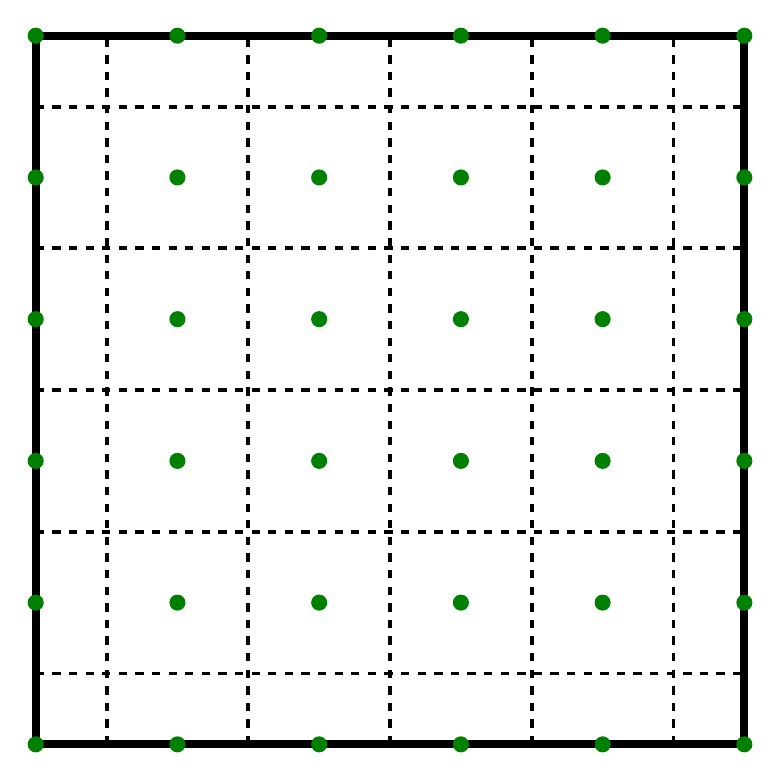
\begin{tikzpicture}[scale=0.9]
    \def\Lx{10cm}
    \def\Ly{10cm}
    \def\velocitylength{1.5cm}
    \draw[line width=1mm] (0,0) rectangle (\Lx,\Ly);

    % Nodes
    \foreach \x in {0,...,5} {
        \foreach \y in {0,...,5} {
            \filldraw[green!50!black] (2*\x,2*\y) circle (3pt);
        }
    }

    \begin{scope}[shift={(1,0)}]
        \foreach \x in {0,...,4} {
            \draw[line width=0.5mm, dashed] (2*\x,0) -- ++(0,\Ly);
        }
    \end{scope}

    % Control volume boundaries y
    \begin{scope}[shift={(0,1)}]
        \foreach \y in {0,...,4} {
            \draw[line width=0.5mm, dashed] (0,2*\y) -- ++(\Lx,0);
        }
    \end{scope}
\end{tikzpicture}
    \caption*{Pressió: cares centrades.}
    \vspace{0.7cm}
    \begin{tikzpicture}[scale=0.9]
    \def\Lx{10cm}
    \def\Ly{10cm}
    \def\velocitylength{1.5cm}

    \fill[black!50!white, opacity=0.5] (-1,-1) rectangle (\Lx + 1 cm,\Ly + 1 cm);
    \fill[white] (0,0) rectangle (\Lx,\Ly);

    \draw[line width=1mm] (0,0) rectangle (\Lx,\Ly);

    % Nodes
    \foreach \x in {0,...,5} {
        \foreach \y in {0,...,5} {
            \filldraw[green!50!black] (2*\x,2*\y) circle (3pt);
        }
    }

    % Control volumes boundaries
    \begin{scope}[shift={(-1,-1)}]
        \foreach \x in {0,...,6} {
            \draw[line width=0.5mm, dashed] (2*\x,0) -- ++(0,\Ly+2cm);
        }
        \foreach \y in {0,...,6} {
            \draw[line width=0.5mm, dashed] (0,2*\y) -- ++(\Lx+2cm,0);
        }
    \end{scope}

    % Velocity u
    \begin{scope}[shift={(1,0)}]
        \foreach \x in {-1,...,5} {
            \foreach \y in {0,...,5} {
                \draw[velocity, line width=0.5mm] ({2*\x cm - 0.5*\velocitylength},2*\y) -- ++(\velocitylength,0);
            }
        }
    \end{scope}

    % Velocity v
    \begin{scope}[shift={(0,-1)}]
        \foreach \x in {0,...,5} {
            \foreach \y in {0,...,6} {
                \draw[velocity, line width=0.5mm, red] (2*\x,2*\y cm - 0.5*\velocitylength) -- ++(0,\velocitylength);
            }
        }            
    \end{scope}
\end{tikzpicture}
    \caption*{Pressió: cares centrades. Velocitat $u$: staggered--$x$. Velocitat $v$: staggered--$y$.}
\end{figure}


\clearpage
\begin{figure}[h]
    \centering
    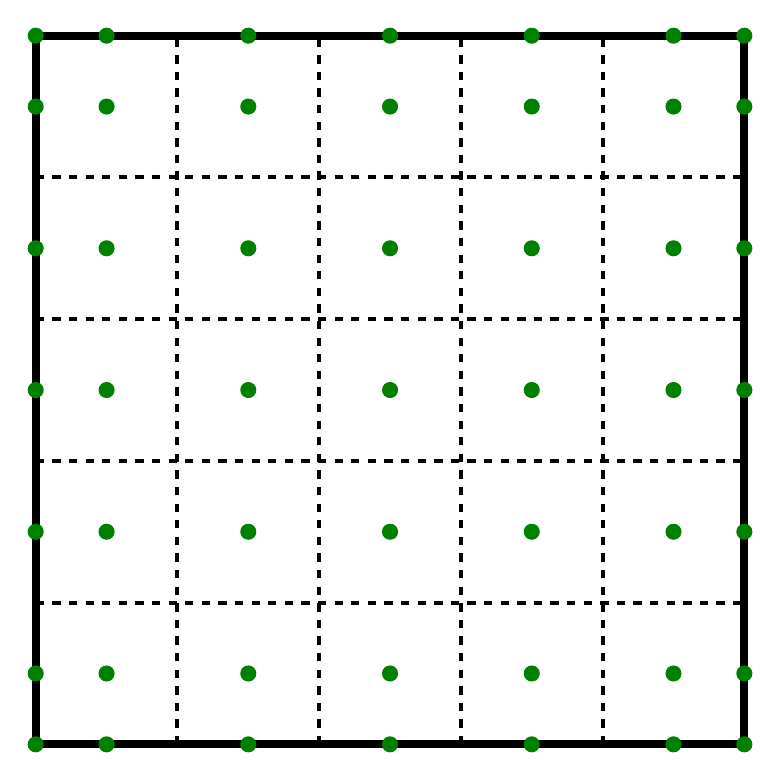
\begin{tikzpicture}[scale=0.9]
    \def\Lx{10cm}
    \def\Ly{10cm}
    \def\velocitylength{1.5cm}
    \draw[line width=1mm] (0,0) rectangle (\Lx,\Ly);

    % Control volume boundaries
    \foreach \x in {1,...,4} {
        \draw[line width=0.5mm, dashed] (2*\x,0) -- ++(0,\Ly);
    }

    \foreach \y in {1,...,4} {
        \draw[line width=0.5mm, dashed] (0,2*\y) -- ++(\Lx,0);
    }

    % Nodes
    \begin{scope}[shift={(1,0)}]
        \foreach \x in {0,...,4} {
            \foreach \y in {0,...,4} {
                \filldraw[green!50!black] (2*\x,2*\y cm + 1 cm) circle (3pt);
            }
        }
    \end{scope}

    % Boundary nodes
    \foreach \y in {0,1} {
        \filldraw[green!50!black] (0,\y*\Ly) circle (3pt);
        \filldraw[green!50!black] (\Lx,\y*\Ly) circle (3pt);
        \begin{scope}[shift={(1,0)}]
            \foreach \x in {0,...,4} {
                \filldraw[green!50!black] (2*\x,\y*\Ly) circle (3pt);
            }
        \end{scope}
    }
    \begin{scope}[shift={(0,1)}]
        \foreach \x in {0,1} {
            \foreach \y in {0,...,4} {
                \filldraw[green!50!black] (\x*\Lx,2*\y cm) circle (3pt);
            }
        }
    \end{scope}

\end{tikzpicture}
    \caption*{Pressió: nodes centrats.}
    \vspace{0.7cm}
    \begin{tikzpicture}[scale=0.9]
    \def\Lx{10cm}
    \def\Ly{10cm}
    \def\velocitylength{1.5cm}
    \draw[line width=1mm] (0,0) rectangle (\Lx,\Ly);

    % Control volume boundaries
    \foreach \x in {1,...,4} {
        \draw[line width=0.5mm, dashed] (2*\x,0) -- ++(0,\Ly);
    }

    \foreach \y in {1,...,4} {
        \draw[line width=0.5mm, dashed] (0,2*\y) -- ++(\Lx,0);
    }

    % Nodes
    \begin{scope}[shift={(1,0)}]
        \foreach \x in {0,...,4} {
            \foreach \y in {0,...,4} {
                \filldraw[green!50!black] (2*\x,2*\y cm + 1 cm) circle (3pt);
            }
        }
    \end{scope}

    % Boundary nodes
    \foreach \y in {0,1} {
        \filldraw[green!50!black] (0,\y*\Ly) circle (3pt);
        \filldraw[green!50!black] (\Lx,\y*\Ly) circle (3pt);
        \begin{scope}[shift={(1,0)}]
            \foreach \x in {0,...,4} {
                \filldraw[green!50!black] (2*\x,\y*\Ly) circle (3pt);
            }
        \end{scope}
    }
    \begin{scope}[shift={(0,1)}]
        \foreach \x in {0,1} {
            \foreach \y in {0,...,4} {
                \filldraw[green!50!black] (\x*\Lx,2*\y cm) circle (3pt);
            }
        }
    \end{scope}

    % Velocity u
    \foreach \y in {0,1} {
        \foreach \x in {0,...,5} {
            \draw[velocity, line width=0.5mm] (2*\x cm -0.5*\velocitylength,\y*\Ly) -- ++(\velocitylength,0);
        }
    }
    \begin{scope}[shift={(0,1)}]
        \foreach \y in {0,...,4} {
            \foreach \x in {0,...,5} {
                \draw[velocity, line width=0.5mm] (2*\x cm -0.5*\velocitylength,2*\y) -- ++(\velocitylength,0);
                
            }
        }
    \end{scope}

    % Velocity v
    \foreach \x in {0,1} {
        \foreach \y in {0,...,5} {
            \draw[velocity, line width=0.5mm, red] (\x*\Lx,2*\y cm - 0.5*\velocitylength) -- ++(0,\velocitylength);
        }
    }
    \begin{scope}[shift={(1,0)}]
        \foreach \x in {0,...,4} {
            \foreach \y in {0,...,5} {
                \draw[velocity, line width=0.5mm, red] (2*\x,2*\y cm - 0.5*\velocitylength) -- ++(0,\velocitylength);
            }
        }
    \end{scope}

\end{tikzpicture}
    \caption*{Pressió: nodes centrades. Velocitat $u$: staggered--$x$. Velocitat $v$: staggered--$y$.}
\end{figure}


>>>>>>> Changes in report. Changes in code: redefinition of surfX, surfY, vol
